\documentclass[border=12pt]{standalone}
\usepackage{amsmath}
\usepackage{tikz}
\usetikzlibrary{arrows.meta}
\usepackage{xcolor}
\definecolor{weeknavy}{HTML}{243B53}
\definecolor{weekblue}{HTML}{6E8FB3}
\definecolor{weeksage}{HTML}{7AA69B}
\definecolor{weekochre}{HTML}{C7A35A}
\begin{document}
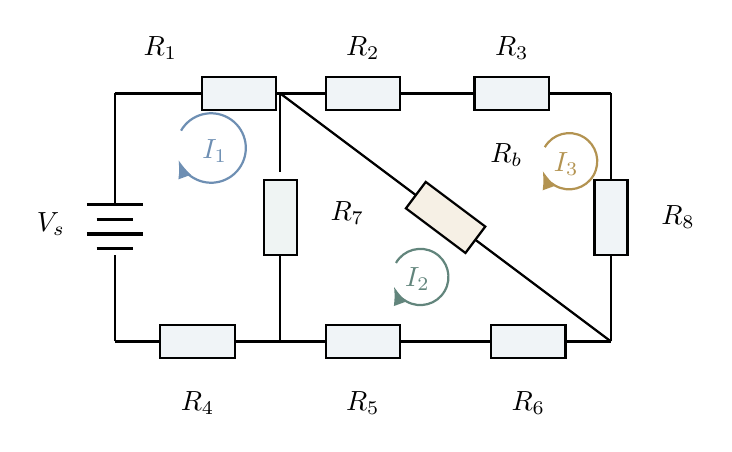
\begin{tikzpicture}[>=Latex,thick,scale=1.05]
% Bridge-style network: three bounded mesh regions, no numerical values.
\draw (0,0)--(0,1.05);
\draw[line width=1.1pt] (-0.22,1.12)--(0.22,1.12);
\draw[line width=1.1pt] (-0.34,1.30)--(0.34,1.30);
\draw[line width=1.1pt] (-0.22,1.48)--(0.22,1.48);
\draw[line width=1.1pt] (-0.34,1.66)--(0.34,1.66);
\draw (0,1.66)--(0,3);
\draw (0,0)--(2,0)--(4,0)--(6,0);
\draw (0,3)--(1.05,3);
\draw[fill=weekblue!10] (1.05,2.80) rectangle (1.95,3.20);
\draw (1.95,3)--(2.55,3);
\draw[fill=weekblue!10] (2.55,2.80) rectangle (3.45,3.20);
\draw (3.45,3)--(6,3);
\draw[fill=weekblue!10] (4.35,2.80) rectangle (5.25,3.20);
\draw (5.25,3)--(6,3);
\draw[fill=weekblue!10] (0.55,-0.20) rectangle (1.45,0.20);
\draw (1.45,0)--(2,0);
\draw[fill=weekblue!10] (2.55,-0.20) rectangle (3.45,0.20);
\draw (3.45,0)--(4,0);
\draw[fill=weekblue!10] (4.55,-0.20) rectangle (5.45,0.20);
\draw (5.45,0)--(6,0);
\draw (2,3)--(2,2.05);
\draw[fill=weeksage!12] (1.80,1.05) rectangle (2.20,1.95);
\draw (2,1.05)--(2,0);
\draw (6,3)--(6,0);
\draw[fill=weekblue!10] (5.80,1.05) rectangle (6.20,1.95);
% The bridge branch follows the diagonal and its resistor is rotated with it.
\draw (2,3)--(6,0);
\begin{scope}[shift={(4,1.5)},rotate=-36.87]
  \draw[fill=weekochre!16] (-0.45,-0.20) rectangle (0.45,0.20);
\end{scope}
% Keep each clockwise mesh arrow inside its actual face.
\draw[->,weekblue] (0.80,2.55) arc[start angle=150,end angle=-160,radius=0.42] node[midway,left=3pt] {$I_1$};
\draw[->,weeksage!80!black] (3.40,0.95) arc[start angle=150,end angle=-160,radius=0.34] node[midway,left=3pt] {$I_2$};
\draw[->,weekochre!90!black] (5.20,2.35) arc[start angle=150,end angle=-160,radius=0.34] node[midway,left=3pt] {$I_3$};
\draw (0.55,3.28) node[above] {$R_1$};
\draw (3.00,3.28) node[above] {$R_2$};
\draw (4.80,3.28) node[above] {$R_3$};
\draw (1.00,-0.48) node[below] {$R_4$};
\draw (3.00,-0.48) node[below] {$R_5$};
\draw (5.00,-0.48) node[below] {$R_6$};
\draw (2.35,1.55) node[right=4pt] {$R_7$};
\draw (6.35,1.50) node[right=4pt] {$R_8$};
\draw (4.35,1.92) node[above right=2pt] {$R_b$};
\draw (-0.48,1.42) node[left] {$V_s$};
\end{tikzpicture}
\end{document}
